\section{Intervention Locations}
\label{sec:accessing_records}

\begin{figure*}[t]
	\centering
	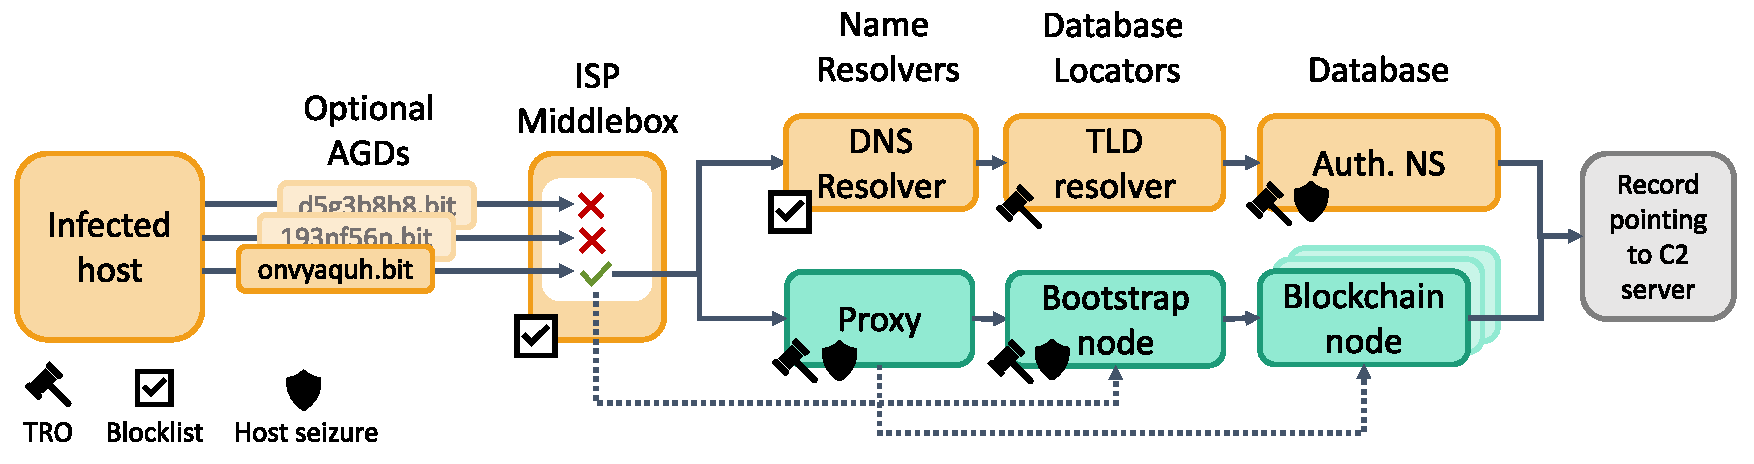
\includegraphics[width=\textwidth]{figs/intervention_locations.pdf}
	\caption{Potential locations of interventions for 
	blocking access to DNS-based and blockchain-based C2 
	server names.}
	\label{fig:malware_contacting_cnc}
\end{figure*}

We have established that malware requires a naming layer to access its C2 
centers, and 
that blockchain-based naming systems are attractive options for implementing 
such a naming layer. We have also examined five naming 
systems individually. 
We now argue that all blockchain-based naming systems share 
certain common 
challenges, and the way these systems overcome these challenges presents 
different advantages or disadvantages for defenders. The first 
of these fundamental challenges is accessing the blockchain.

Accessing any distributed, peer-to-peer system for the first time requires 
learning the address of at least one participating node. In general, there 
are two methods for finding such an address: connecting to a 
proxy that already knows how to reach a member of the system, or acting 
as a full member of the system and utilizing its peer-to-peer discovery 
protocol. The latter approach requires knowing a list of ``bootstrap nodes.'' 
For example, Ethereum uses a list of bootstrap nodes that are hard-coded into 
client implementations~\cite{geth_bootstrap}. Bitcoin 
stores lists of bootstrap nodes in DNS TXT records maintained by volunteers, as 
well as hard-coded 
lists~\cite{bitcoin_bootstrap}. A third option, a 
local discovery protocol that floods the network with 
messages looking for nodes, has not been adopted by any 
blockchains that we are aware of. Such an approach would only be successful if 
nodes running the blockchain were present on most networks. 
 
Figure~\ref{fig:malware_contacting_cnc} compares the steps an infected host 
takes to resolve a DNS C2 domain to the steps required to resolve a blockchain 
name. It also details the interventions that can be taken by defenders at each 
step. We now describe each step in detail.

\subsection{Reaching the resolver}

Regardless of whether a request is destined for DNS or a blockchain naming 
system, it must first reach the machine that acts as a resolver: either the DNS 
resolver or the proxy in Figure~\ref{fig:malware_contacting_cnc}. Defenders may 
be able to intervene before this point by placing middleboxes with filter lists 
in the network. Some networks already have such defenses: for example, some ISP 
networks redirect all DNS requests to the ISP's own resolver, which can 
implement a filter list. This defense is probably not currently intended to 
block blockchain names, but it works by chance in some cases. Some malware uses 
ordinary DNS rather than DNS-over-HTTPS to request blockchain domains, under 
the assumption that the proxy the query is intended for will redirect it to the 
blockchain naming system in the correct format. When ISPs perform DNS 
redirection to their own resolvers, these queries get redirected to the DNS 
root, which cannot resolve the alt-TLDs used by blockchain naming systems. We 
present our study of this phenomenon in Section~\ref{sec:b-root}. We observe 
that filter lists are only a partial defense against malware, because malware 
may utilize DGAs to evade them. 

\subsection{Interventions at the name resolver}

When using blockchain naming systems, the entity that first attempts to resolve 
a request is a proxy rather than a pure DNS resolver. It may expect queries in 
the form of DNS-over-HTTPS, unencrypted DNS, or in an 
arbitrary format. Instead of querying the DNS root zone, the 
TLD resolver, and eventually the authoritative nameserver to 
resolve a name, the proxy must connect to the blockchain and 
retrieve the record from one of the participants.
Defenders may intervene at a traditional DNS resolver by requesting that the 
resolver implement a filter list, or the resolver operators may elect to 
implement one voluntarily. However, proxies that resolve blockchain names may 
be resistant to such voluntary efforts, because proxy 
operators often identify with the libertarian values 
associated with the goals of blockchain. 


Proxies are currently the most common method for resolving 
blockchain names. Table~\ref{tab:proxies_and_tlds} shows a 
selection of the proxies and tools that resolve names from 
each of the systems we study. The list of proxies is not 
exhaustive, but represents 
a subset of the best-known proxies in use at the time of 
writing. While most large 
browsers, such as Safari, Chrome, and Firefox, do not support 
any blockchain naming systems natively, some naming systems 
provide browser extensions that redirect blockchain name 
queries to proxies using DoH. A few browsers do resolve 
blockchain names without requiring extensions, such as Brave, 
which partners with a proxy called 
Infura~\cite{brave_uses_infura}. Some naming systems have 
partnerships with existing DNS resolvers. For example, 
NextDNS's DNS resolvers can act as proxies to resolve 
Handshake names. Finally, some naming systems, such as 
Handshake, also provide stub resolver implementations that 
run locally on a user's computer. These stub resolvers also 
work by routing blockchain name queries to proxies.

All of these proxies are centralized, in that they 
are controlled by a single authority. This is good 
news for defenders: similarly to traditional registrars, they 
are vulnerable to legal takedowns. They can be served with 
TROs or warrants and compelled to stop giving access to 
abused domains, as long as they operate within a jurisdiction 
amenable to such efforts. A centralized proxy could also be 
neutralized by serving a takedown order to its 
hosting provider, although this approach would produce 
varying amounts of the collateral damage depending on how 
many licit users utilize the proxy. 
While these interventions are not 
foolproof, they are subject to the same advantages and 
disadvantages as interventions on traditional registrars. 
Thus, centralized proxies return the distributed naming 
ecosystem to a state similar to the DNS ecosystem, from a 
defender's point of view. 
%We conclude that proxy takedowns 
%are a viable method for 
%defenders to intervene in the blockchain DNS ecosystem. 
However, while proxies greatly simplify the process of 
connecting to a blockchain, they are not strictly necessary, 
which is bad news for defenders.

\subsection{Skipping the proxy: the rise of light clients}

We initially assumed that no infected host would be able to 
skip the proxy and participate directly 
in the blockchain, because acting as a blockchain node 
requires too many resources. However, this assumption turned 
out to be incorrect, because of the rise of \emph{light 
clients}. When blockchains were first envisioned, most 
assumed that every participant in the network would be a 
``full'' implementation of a node: it would contain 
enough state to reconstruct the entire history of the chain, 
all the way back to the first transaction. Additionally, each 
node would contribute to the 
blockchain by verifying every transaction it heard about. As 
blockchains grow over time, they become too 
resource-intensive to run on anything other than a dedicated, 
powerful machine. Two resources serve as 
the constraints: first, CPU power, which is obviously 
necessary to perform mining but now is even a bottleneck for 
transaction verification, because so many transactions happen 
per second~\cite{citation_needed}. Second, disk 
space and speed. For example, a full Ethereum node cannot be 
run on a machine with a hard disk drive anymore, because 
nothing slower than an SSD can keep up with the 
reads and writes required~\cite{citation_needed}. These 
resource constraints make it 
very unlikely that malware could run ``full'' blockchain 
nodes on infected hosts. However, these constraints have also
given rise to the concept of a ``light client,'' a blockchain 
node with limited functionality that can fetch transactions 
from the chain but does not contribute by verifying 
transactions, mining, or broadcasting. Light clients are 
designed to run on laptops and mobile devices. As such, they 
use few enough resources to reasonably be included in 
malware. 


\subsection{Interventions at the Database Locator}

Light clients enable malware to act as a first-class member 
of a blockchain, and discover other members of the chain 
using the chain's peer-to-peer discovery protocol without 
using a centralized proxy. In this case, defenders are left 
with a harder location to stage an intervention: the 
blockchain's bootstrap nodes, which is the blockchain 
equivalent of a service that locates the database of naming 
records.

%Most peer-to-peer discovery 
%protocols allow a client to connect to the blockchain for 
%the 
%first time by hard-coding a set of ``bootstrap nodes.'' In 
%Ethereum, these bootstrap nodes are hard-coded into various 
%implementations of the clients, and in Bitcoin, they are 
%either hard-coded or accessible as TXT records stored at 
%various trusted domains. The list of bootstrap nodes may 
%also 
%be configured by the user. If the 
%malware chooses to use the bootstrap nodes that are 
%hard-coded by default into the light client implementation, 
%this may present a challenge for defenders, because taking 
%down those bootstrap nodes may cause collateral damage to 
%legitimate users attempting to join the chain. As such, 
%bootstrap nodes are a more difficult place to stage an 
%effective defender intervention than centralized proxies. 


In traditional DNS, the resolver must locate the database 
that contains a record by first querying the hierarchy of DNS 
servers: first the root and then the TLD resolver. The TLD 
resolver's role is to tell the DNS resolver which machine 
stores the database that ultimately contains a name's 
records. In a blockchain system, this role is filled by the 
blockchain's bootstrap nodes, which are publicly listed 
nodes that maintain connections to some of the other 
participants in the blockchain. The purpose of the bootstrap 
nodes is to provide a gateway to the blockchain for new 
participants: new blockchain nodes find their initial list of 
potential peers by connecting to the bootstrap nodes.

When defenders perform interventions by putting legal 
pressure on registrars, the intervention takes effect at the 
TLD resolver, which implements the changes to the zone file 
that affect the malware's domains. These changes can include 
``sinkholing'' the domain by causing it resolve to an IP 
controlled by defenders or ``freezing'' it so that 
its records cannot be modified. This intervention does not 
translate well to blockchain naming systems for several 
reasons. 

First, while bootstrap nodes are responsible for finding the 
entire naming database, they do not allow defenders to 
specify which blockchain systems a client may access and 
which it may not. This means that seizing a specific naming 
record, or even the entire naming system, is not possible at 
the bootstrap nodes. Consequently, disabling or seizing 
bootstrap nodes prevents all new clients from accessing any 
functionality provided by the blockchain, including the 
blockchain's cryptocurrencies and any services it offers 
unrelated to naming. This approach therefore carries the 
potential for a lot of collateral damage. Second, bootstrap 
nodes may be widely distributed across the globe, leading to 
jurisdictional challenges in bringing legal pressure to bear 
on their operators. Bootstrap nodes may also be difficult to 
find, since they may not be run by hosting providers but 
rather by anonymous individual volunteers. Third, bootstrap 
nodes may be numerous enough that finding and seizing them 
all may be prohibitively difficult. Finally, while the 
default bootstrap node lists are published for each 
blockchain, users may choose to substitute their own. A 
malware author could design a payload that contains an 
extensive list of machines that participate in a blockchain 
naming system, which would complicate a defender's efforts to 
take down all the potential participants. 

However, defenders could fall back to a blocklist-based 
approach to deny access to bootstrap nodes. For example, 
IDSes, enterprise firewalls, or ISP routers can drop traffic 
intended for bootstrap nodes. This approach is very similar 
to blocking any other 
malicious IP addresses, and is subject to the usual 
challenges. Defenders must keep blocklists up-to-date as 
malware authors update the IPs they connect to. To the 
advantage of defenders, any time malware authors 
are forced to update the IP addresses that bootstrap nodes 
may be found at, they run afoul of the ``sunk cost'' problem 
where infected machines that cannot be updated become
useless. A similar argument applies if malware chooses to 
access bootstrap nodes using hard-coded DNS domain names 
instead of hard-coded IP addresses. Additionally, 
traditional interventions against domain names apply in that 
situation as well. Thus, while intervening at bootstrap nodes 
poses more of a challenge than intervening at centralized 
proxies, defenders still have viable options to choose from.

\subsection{Interventions at the Database}

In traditional DNS, defenders can sinkhole the domain of an 
authoritative nameserver or seize the server itself to 
prevent malware accessing a C2 domain record. This 
intervention is impractical for blockchain names, 
because instead of a single machine acting as the 
authoritative nameserver, every blockchain node has a copy of 
the database. Seizing the database would require either taking down 
every machine in the blockchain, or executing a successful ``51\%'' attack by 
taking control of more than half of the computing power in the blockchain. 
Blockchains are generally highly robust against attacks like these, which makes 
them unlikely to be the most practical intervention for defenders to attempt. 
However, small naming-specific
blockchains with few participants may be more vulnerable --- see 
Section~\ref{sec:namecoin_51}.

\subsection{Interventions after the name record is acquired}
\label{sec:interventions_at_name}

If an infected host successfully retrieves its C2 record, 
that record might take several forms. The three that we 
observed in existing blockchain naming systems that might be 
useful to malware were IP addresses, traditional DNS domains, 
and addresses for distributed storage systems like IPFS and 
SkyNet. We refer to these addresses as ``distributed 
storage'' (DS) addresses from this point forward. Some naming 
systems also allow users to store arbitrary text as 
records, which would let malware operators store nonstandard 
record types like links to social media posts. 

Each of these record types are subject to all of the 
traditional interventions that have already 
been described, except one: DS addresses. Distributed storage 
systems provide a form of ``bulletproof'' hosting, under the limitation
that all hosted content must be static files and not dynamic 
websites. Any C2 server implemented entirely on such a 
system must be a simple file with no 
dynamic content. Infected hosts that wish to contact a distributed storage 
system must pass through the same steps shown in 
Figure~\ref{fig:malware_contacting_cnc} for accessing a blockchain, which means 
they are subject to the same interventions. For example, a strain of malware 
called ``IPStorm'' has already been discovered using IPFS for its C2 server in 
the wild. IPStorm connects to IPFS using bootstrap nodes~\cite{ipstorm_anomali, 
ipstorm_zdnet}, which may be seized or blocked.

Another advantage for defenders is that some distributed storage systems, 
such as IPFS, do not have redundancy: only a single machine hosts each piece of 
a file. This raises the possibility of discovering the particular machine 
responsible for hosting a C2 server and seizing it. 

A final possibility for intervening with the name record may be to seize 
names stored in ``hosted'' or ``custodial'' wallets. Businesses such 
as cryptocurrency exchanges provide custodial wallets for users who wish to let 
the company handle their blockchain-based assets. This service is designed to 
make blockchain interaction easier for customers, but as a consequence, the 
business knows the custodial wallet's private key. If a name is stored in a 
custodial wallet, the business that runs the wallet 
could seize it~\cite{pegoraro_blockchain_2021}. However, a 
successful intervention must be difficult for malware operators to 
evade, and we note that malware operators with good operational practices can 
simply choose not to use custodial wallets. 

\subsection{Intervening with name modification or purchase}

Generally speaking, DNS domains are cheaper, easier to modify, and 
easier to replace than IP addresses, because each IP address 
represents a compromised machine while new domains can be 
purchased inexpensively. Blockchain-based domains on 
general-purpose chains, such as Bitcoin and Ethereum, 
change this norm. While resolving a name is free, malware 
operators must pay \emph{transaction fees} 
(known as \emph{``gas fees''} on Ethereum)
to register or modify names. These transaction fees 
can be quite expensive. For example, we found that 
registering a new name on the Unstoppable Domains service 
cost nearly \$80 in gas fees during a period of high fees. 
In contrast, the cost of the name itself was \$10. While 
licit users may wait for fees to be low at times of low 
network congestion, malware operators may not have that 
choice if they wish to avoid downtime in their campaign. High 
transaction costs poses challenges for defenders as well. For 
example, to combat DNS-based DGAs, defenders have the option 
of registering every domain the DGA will ever generate. This 
intervention would be much less practical if each 
registration was nearly an order of magnitude more expensive.

Naming-specific blockchains, such as Namecoin, Emercoin, and Handshake, 
present a different set of tradeoffs for defenders and malware 
operators. These 
blockchains are created with the sole intention of hosting a naming system. 
With fewer users and correspondingly less demand, these systems' names are 
usually much less expensive than names in Ethereum-based systems. This enables 
malware authors to use fast flux or DGA-based strategies, and also may enable 
defenders to pre-register domains generated by DGAs. 






%\subsection{Naming record formats}
%
%
%
%
%\randall{where do I put this? Additionally, because all 
%blockchain 
%	records 
%	are public, anyone can fetch those records including 
%	defenders. You could theoretically scrape a blockchain 
%looking for records 
%	that match a known 
%	malicious format or with malicious traits of some sort 
%(owned by the same 
%	wallet?) and try to seize 
%	whatever those records point to.} 
%
%
%
%I don't know if IPFS/SkyNet have light nodes that could be 
%part of a malware payload, but there does seem to be a trend 
%in that direction as chains get heavier.